\section{Solution Overview}
This section provides an overview of the approach and explains how it addresses requirements R1 to R3.
A visualization of the approach is shown in Fig. \ref{fig:solution-overview}. As mentioned in Requirement R1, the approach shall apply to existing applications, and they should be able to support run-time state migration. For ease of enabling existing applications, we chose to develop some necessary libraries. These libraries shall provide an API for validation, injection, and extraction states. As stated in \textbf{Requirement R2}, the approach shall enable the ability of state management. Thereby, modeling the state is possible by DSL, which will be integrated with special libraries.

Besides libraries, our approach needs device management and device discovery which is stated in \textbf{Requirement R3}. Middleware serves as device management, allowing devices to introduce themselves and allows devices to find each other and get noticed when a device joined or left. Also, if devices are in the same local network, these libraries establish a point-to-point connection. Otherwise, they use middleware to communicate over the internet to migrate the run-time state.

\begin{figure}[!b]
    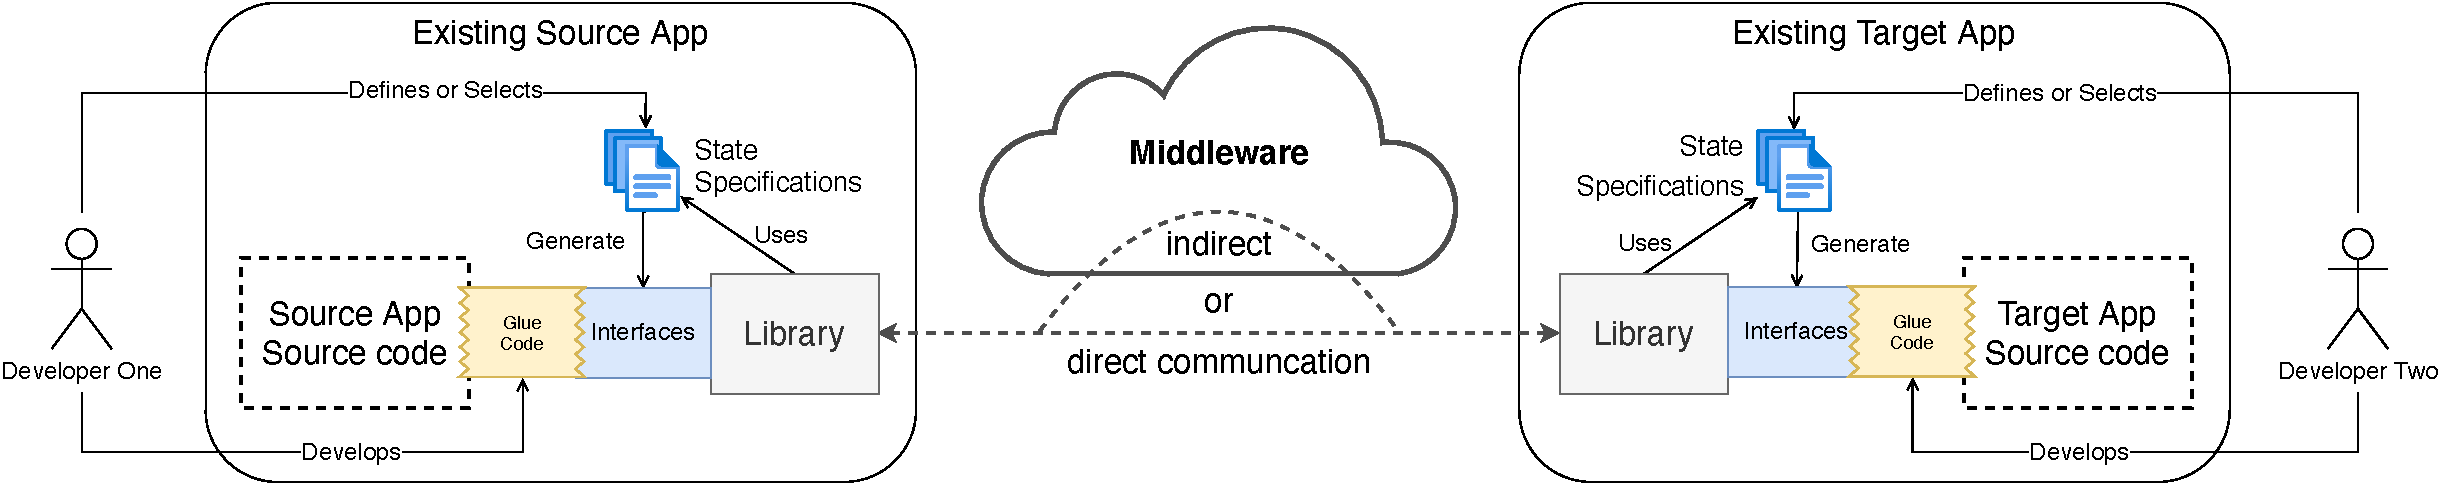
\includegraphics[width=\linewidth]{../figures/solution-overview}
    \centering
    \caption{General overview of the approach}
    \label{fig:solution-overview}
\end{figure}
